\documentclass{slides}
\title{Drivetrain Update Flow}
\author{Natan Jurca}
\date{September 2025}

\usepackage{tikz}
\usetikzlibrary{shapes.geometric, arrows}
\usetikzlibrary{positioning}

\tikzstyle{startstop} = [rectangle, rounded corners, minimum width=3cm, minimum height=1cm,text centered, draw=black, fill=red!30]
\tikzstyle{io} = [trapezium, trapezium left angle=70, trapezium right angle=110, minimum width=3cm, minimum height=1cm, text centered, draw=black]
\tikzstyle{process} = [rectangle, minimum width=3cm, minimum height=1cm, text centered, draw=black]
\tikzstyle{decision} = [diamond, aspect=2, minimum width=3cm, minimum height=1cm, text centered, draw=black]
\tikzstyle{big_decision} = [diamond, aspect=4, minimum width=3cm, minimum height=1cm, text centered, draw=black]
\tikzstyle{arrow} = [thick,->,>=latex]

\begin{document}
\resizebox{!}{20cm}{%
	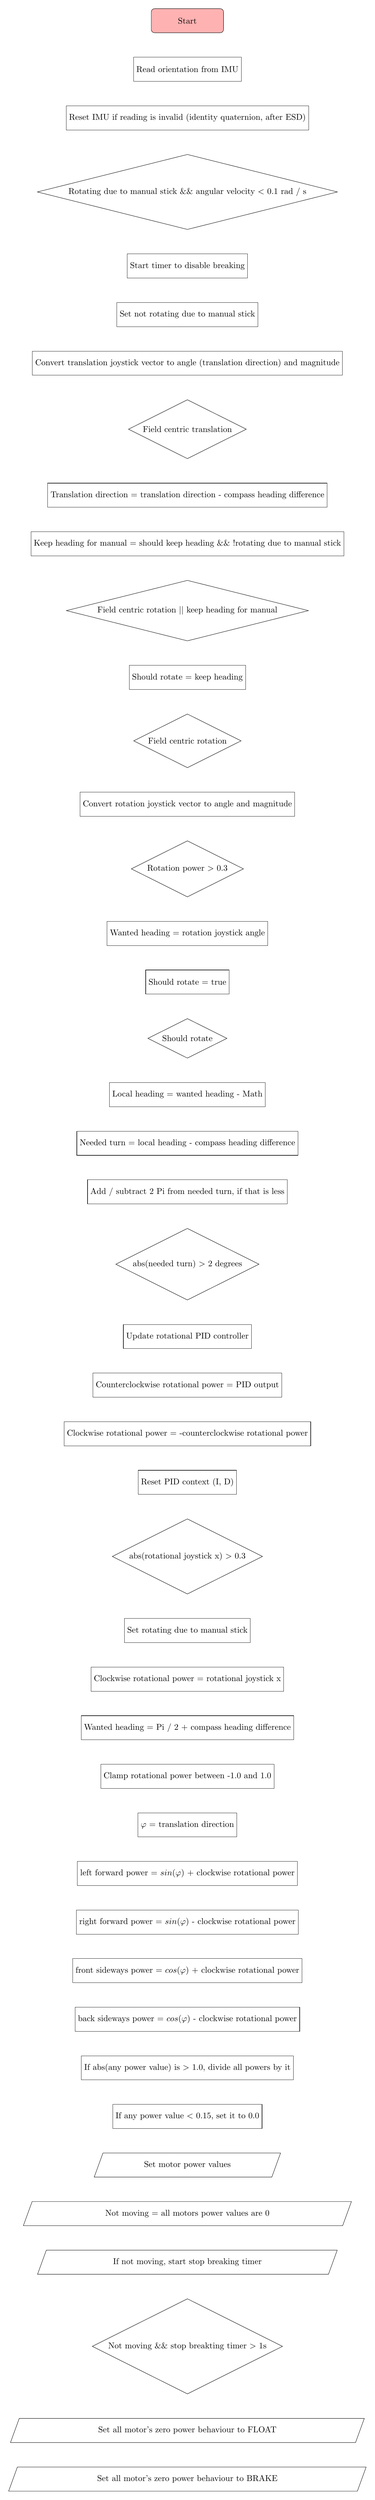
\begin{tikzpicture}[node distance=1cm]
		\node (start) [startstop] {Start};
		\node (read_from_imu) [process, below=of start] {Read orientation from IMU};
		\node (fix_imu) [process, below=of read_from_imu] {Reset IMU if reading is invalid (identity quaternion, after ESD)};

		\node (stop_manual_rotation_if) [big_decision, below=of fix_imu] {Rotating due to manual stick \&\& angular velocity $<$ 0.1 rad / s};

		\node (start_break_time) [process, below=of stop_manual_rotation_if] {Start timer to disable breaking};
		\node (not_rotating_due_to_manual_stick) [process, below=of start_break_time] {Set not rotating due to manual stick};
		\node (get_magnitude_and_phi_for) [process, below=of not_rotating_due_to_manual_stick] {Convert translation joystick vector to angle (translation direction) and magnitude};

		\node (field_centric_translation_if) [decision, below=of get_magnitude_and_phi_for] {Field centric translation};

		\node (compensate_for_heading_difference) [process, below=of field_centric_translation_if] {Translation direction = translation direction - compass heading difference};
		\node (keep_heading_for_robot_centric) [process, below=of compensate_for_heading_difference] {Keep heading for manual = should keep heading \&\& !rotating due to manual stick};

		\node (field_centric_translation_if) [big_decision, below=of keep_heading_for_robot_centric] {Field centric rotation $||$ keep heading for manual};

		\node (should_rotate) [process, below=of field_centric_translation_if] {Should rotate = keep heading};

		\node (if_field_centric_rotatiom) [decision, below=of should_rotate] {Field centric rotation};
		\node (get_magnitude_and_phi_for_rotation) [process, below=of if_field_centric_rotatiom] {Convert rotation joystick vector to angle and magnitude};

		\node (if_rotation_power_enough) [decision, below=of get_magnitude_and_phi_for_rotation] {Rotation power $>$ 0.3};
		\node (update_wanted_heading) [process, below=of if_rotation_power_enough] {Wanted heading = rotation joystick angle};
		\node (update_should_rotate_fcr) [process, below=of update_wanted_heading] {Should rotate = true};

		\node (if_should_rotate) [decision, below=of update_should_rotate_fcr] {Should rotate};
		\node (wanted_heading_local) [process, below=of if_should_rotate] {Local heading = wanted heading - Math};

		\node (needed_turn) [process, below=of wanted_heading_local] {Needed turn = local heading - compass heading difference};
		\node (needed_turn_faster) [process, below=of needed_turn] {Add / subtract 2 Pi from needed turn, if that is less};

		\node (if_needed_turn_more_than_minimum) [decision, below=of needed_turn_faster] {abs(needed turn) $>$ 2 degrees};
		\node (rotation_pid) [process, below=of if_needed_turn_more_than_minimum] {Update rotational PID controller};

		\node (rotation_pid_2) [process, below=of rotation_pid] {Counterclockwise rotational power = PID output};
		\node (rotation_pid_3) [process, below=of rotation_pid_2] {Clockwise rotational power = -counterclockwise rotational power};

		\node (rotation_pid_reset) [process, below=of rotation_pid_3] {Reset PID context (I, D)};

		\node (if_manual_rotation_power_enough) [decision, below=of rotation_pid_reset] {abs(rotational joystick x) $>$ 0.3};
		\node (update_started_rotating_manually) [process, below=of if_manual_rotation_power_enough] {Set rotating due to manual stick};

		\node (clockwise_rotation_power_stick_x) [process, below=of update_started_rotating_manually] {Clockwise rotational power = rotational joystick x};
		\node (wanted_heading_pi_2) [process, below=of clockwise_rotation_power_stick_x] {Wanted heading = Pi / 2 + compass heading difference};

		\node (clamp_rotational_power) [process, below=of wanted_heading_pi_2] {Clamp rotational power between -1.0 and 1.0};

		\node (set_phi_direction) [process, below=of clamp_rotational_power] {$\varphi$ = translation direction};
		\node (lf_power) [process, below=of set_phi_direction] {left forward power = $sin(\varphi)$ + clockwise rotational power};
		\node (rf_power) [process, below=of lf_power] {right forward power = $sin(\varphi)$ - clockwise rotational power};
		\node (fs_power) [process, below=of rf_power] {front sideways power = $cos(\varphi)$ + clockwise rotational power};
		\node (bc_power) [process, below=of fs_power] {back sideways power = $cos(\varphi)$ - clockwise rotational power};

		\node (normalize_pwrs) [process, below=of bc_power] {If abs(any power value) is $>$ 1.0, divide all powers by it};

		\node (normalize_pwrs_2) [process, below=of normalize_pwrs] {If any power value $<$ 0.15, set it to 0.0};

		\node (set_powers) [io, below=of normalize_pwrs_2] {Set motor power values};

		\node (stopped_moving) [io, below=of set_powers] {Not moving = all motors power values are 0};

		\node (stopped_moving_2) [io, below=of stopped_moving] {If not moving, start stop breaking timer};

		\node (stopped_moving_3) [decision, below=of stopped_moving_2] {Not moving \&\& stop breakting timer $>$ 1s};

		\node (stopped_moving_4) [io, below=of stopped_moving_3] {Set all motor's zero power behaviour to FLOAT};

		\node (stopped_moving_5) [io, below=of stopped_moving_4] {Set all motor's zero power behaviour to BRAKE};
		%
		%\node (stop) [startstop, below=of] {Stop};
	\end{tikzpicture}
}
\end{document}
